\subsection{Decision Trees}

Decision trees are one of the most widely used supervised machine learning algorithms either 
as standalone solutions or in combination with enhancement approaches like boosting. 
They allow for a very flexible construction and can be utilized for various machine learning problems
such as classifcation and regression.

Decision trees “predict an unknown value of a target variable by learning decision rules from 
data features” to reconstruct the dependence between the features and the respective labels for 
each sample. To perform classification or regression, decision trees rely on recursive 
splitting of the dataset into multiple subgroups. As the number of iterations increases, the 
subgroups become more and more homogeneous \cite[p.330]{James2021}. The ideal result is that each subgroup is fully 
homogeneous and therefore only represents a single category (in case of classification). However, 
this is often only a theoretical best condition, as multiple risks, such as overfitting, are 
associated with the increasing depth of decision trees.

Trees consist out of four main components. A node is a discrete decision function that takes 
samples as its input and splits them based on features into subgroups. The aim of each split, 
as previously discussed, is to create a split that results in the overall most homogeneous 
distribution for all subgroups \cite[p.6]{lewis2000introduction}. Nodes can be subclassified into three kinds. The top-node, 
from which the classification starts, is called a root node. Nodes that are located at the 
very end of a decision tree are referred to as leaves. Leaves do not split data any further and 
only mark the end of a decision tree. When reached, leaves categorize or predict a final output 
value depending on the prediction task. Nodes in-between the root node and leaves are called 
internal nodes. Like the root, internal nodes are responsible for the recursive splitting of 
the data. Branches connect Nodes with another. For classical trees, information only flows from 
top to bottom of the tree. 

%In practice, there exist various Algorithms for computing Decision Trees with the most common ones 
%being: ID3, C4.5, C5.0 and \ac{CART}. Each algorithm follows the same principle of regressively finding 
%perfect splits to separate data but utilizes different methods to find the ideal splitting 
%criteria, which strongly influences the structure of the tree, its accuracy and performance. 
%Additionally, each algorithm has its benefits and constraints. Therefore, it is important to 
%determine the best Algorithm before implementing a decision tree based on the prediction task 
%and dataset. This project uses the python library sklearn to implement a classification tree. 
%Sklearn is based on the \ac{CART} algorithm \cite[10.10.6]{sklearn Decision Trees}.

In practice, there exsist various implementations for computing decision trees. Each follows the same 
principle of regressively finding perfect splits to seperate the data but different methods to find 
the ideal splitting criteria, which strongly influences the structure of the tree, its accuracy and 
performance. Thus each implementation has benefits and constraints which have to be taken into account
when determining the model. This project uses the python library sklearn to implement a classification tree. 
Sklearn is based on the \ac{CART} algorithm \cite[10.10.6]{sklearn Decision Trees}.


\subsubsection{Decision Tree Algorithm}

\textbf{Initial Dataset:}

To better visualize the procedure of the decision tree algorithm, a simplified dataset is used, 
on which the individual steps are explained. For this example, a classification problem is chosen. 
The dataset consists out of actual features and labels from the project implementation phase. The 
features are \emph{acousticness} and \emph{danceability}. Both features are numerical with a value range 
in-between \(0\) and \(1\). The classification problem is binary with \emph{hiphop} and \emph{jazz} representing 
the classes \(k\) for which the samples of the dataset are classified. Mathematically, the dataset 
is represented in the following form: \(x_{i}\) presents a set of explanatory features while \(y_{i}\) represents 
the corresponding label for one data point of the input dataset \(N\) with a total number of \(n\) 
samples.

\begin{table}[H]
    \centering
    \begin{tabular}{llrrr}
        \toprule
        category & track &  feature\_danceability &  feature\_acousticness &  label \\
        \midrule
          hiphop &    h1 &                 0.949 &                 0.132 &      1 \\
          hiphop &    h2 &                 0.743 &                 0.234 &      1 \\
          hiphop &    h3 &                 0.913 &                 0.394 &      1 \\
          hiphop &    h4 &                 0.810 &                 0.504 &      1 \\
          hiphop &    h5 &                 0.434 &                 0.198 &      1 \\
            jazz &    j1 &                 0.654 &                 0.534 &      0 \\
            jazz &    j2 &                 0.593 &                 0.312 &      0 \\
            jazz &    j3 &                 0.234 &                 0.341 &      0 \\
        \bottomrule
        \end{tabular}        
    \caption{Theory: Input Data}%
    \label{tbl:theory_input_data}%
  \end{table} 

\textbf{Recursive Tree Construction:} 

The decision tree algorithms splits the dataset recursively into subsets. At the beginning, the whole dataset is 
contained within the root node from which the division into subtrees start. Each node is mathematically described
as \(Q_{m}\) and contains a subgroup \(N_{m}\) of the input dataset. Nodes split their respective groups of data 
further or act as a final classifier in the form of a leaf. The split can be 
binary or multiway. \ac{CART} only utilizes binary splits and divides the Node \(Q_{m}\) into two repective subgroups 
labeled as \(Q^{left}_{m}\) and \(Q^{right}_{m}\). 

The algorithm is greedy and thus determines for each split an optimal division of the samples according to 
the impurity of both subgroups. The goal for every split is to divide the group of data into two subgroups which are 
more homogeneous as the origin and maximize the overall homogenity. The division of the data is 
always performed using a feature, on the basis of which the samples can be divided either by a threshold for 
nominal values or an is-equal-to query for categorical values. The split is mathematically described as the 
following (1). It consists out of the the feature \(j\) and a criteria \(t_{m}\).

\begin{equation}
\theta = (j, t_{m})
\end{equation}

\textbf{Splitting Criteria and Information Gain:}

The optimal split is determined by selecting the feature that has the highest information gain. Information gain 
stands for the knowledge and information about the dependence between features and labels gained by splitting a group 
of samples by a feature. Ideally, the information gain is maximized. Mathematically spoken, the split is optimal if 
the nformation gain \(G(Q_{m}, \theta)\) (2) is minimized as shown in (3). 

\begin{equation}
G(Q_{m},\theta) = \frac{N^{left}_{m}}{N_{m}} H(Q^{left}_{m}, \theta ) + \frac{N^{right}_{m}}{N_{m}} H(Q^{right}_{m}, \theta )
\end{equation}

\begin{equation}
\theta ^* = \arg \min_{\theta}  G(Q_{m}, \theta)
\end{equation}

To determine the overall best \(G(Q_{m}, \theta)\) the respective impurities \(H\) for both subgroups \(Q^{left}_{m}\) 
and \(Q^{right}_{m}\) are required. Each impurity is weighted according to its relative size 
\(\frac{N^{left}_{m}}{N_{m}}\).

The impurity \(H\) for \ac{CART} is calculated by the gini index. Gini index measures the probability that a sample 
does not belong to the category that represents the majority of the subgroup \cite[p.335]{James2021}. If both 
categories of a subgroup are identical in size, the gini index reaches its maximum point at \(0,5\) (figure 1). The 
maximum of the gini index means the worst possible data constellation for a subgroup with maximum heterogeneity. 
Gini index equal to \(0\) on the other hand represents the best possible result with the subgroup being fully 
homogenous. \(p_{i}\) represents that probability that a sample belongs to the class \(j\).

\begin{equation}
Gini = 1 - \sum ^k_{j = 1}(p_{j})^2
\end{equation}

\begin{figure}[H]
    \centering
    \caption[]{Coordinate System}
	\label{fig:coordinate_system_initial_dataset}
    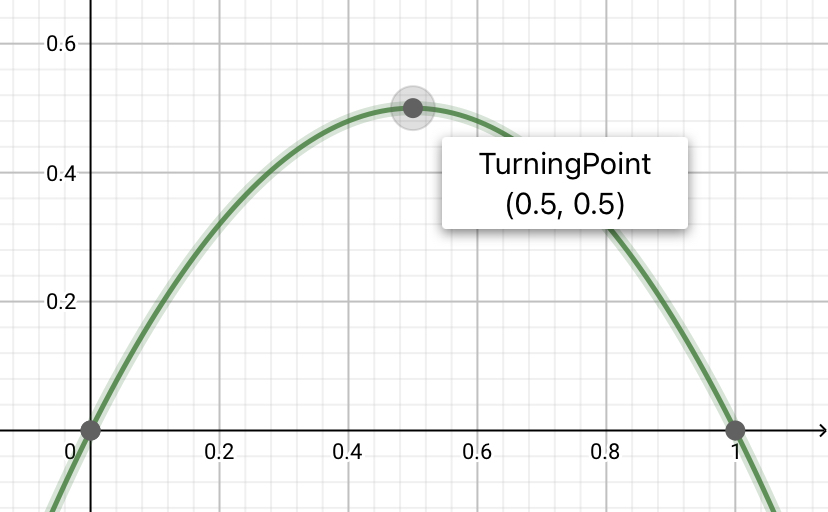
\includegraphics[width=0.5\textwidth]{coordinate_system_gini_index.jpeg}
\end{figure}

The optimal splits for the first iteration of the dataset look like the following. For numerical features the determination of 
the optimal split is more complex as for categorical ones because the the calculation is not straight forward but must be computed
for every value in the value range to find the best overall split for a single feaute. The example only shows the best splitting
criteria is shown while a trial and error approach can be found in the appendix. 

Danceability: 
\begin{equation*}
    \begin{aligned}
        Gini^{left} &= 1 - ((\frac{2}{5})^2 + (\frac{3}{5})^2) = 0,48 
        \\
        Gini^{right}  &= 1 - ((\frac{3}{3})^2 + (\frac{0}{3})^2) = 0 
        \\
        G(Q_{0},\theta) &= \frac{5}{8} * 0,48 + \frac{3}{8} * 0 = 0,30
    \end{aligned}
\end{equation*}

Acousticness: 
\begin{equation*}
    \begin{aligned}
        Gini^{left}  &= 1 - ((\frac{4}{4})^2 + (\frac{0}{4})^2) = 0
        \\
        Gini^{right} &= 1 - ((\frac{1}{4})^2 + (\frac{3}{4})^2) = 0,36
        \\
        G(Q_{0},\theta) &= \frac{4}{8} * 0 + \frac{4}{8} * 0,36 = 0,18
    \end{aligned}
\end{equation*}

The conclusion is that the feature \emph{danceability} creates a bettter initial prediction than \emph{acousticness} does. It is thus 
determined to be the inital splitting criteria for the classification tree (figure 2). With the first iteration completed, the next iteration
will start with each leaf as its input. The second iteration will split the nodes further if no stop criteria is met. 

\begin{figure}[H]
    \centering
    \subfloat[\centering Decision Tree]{{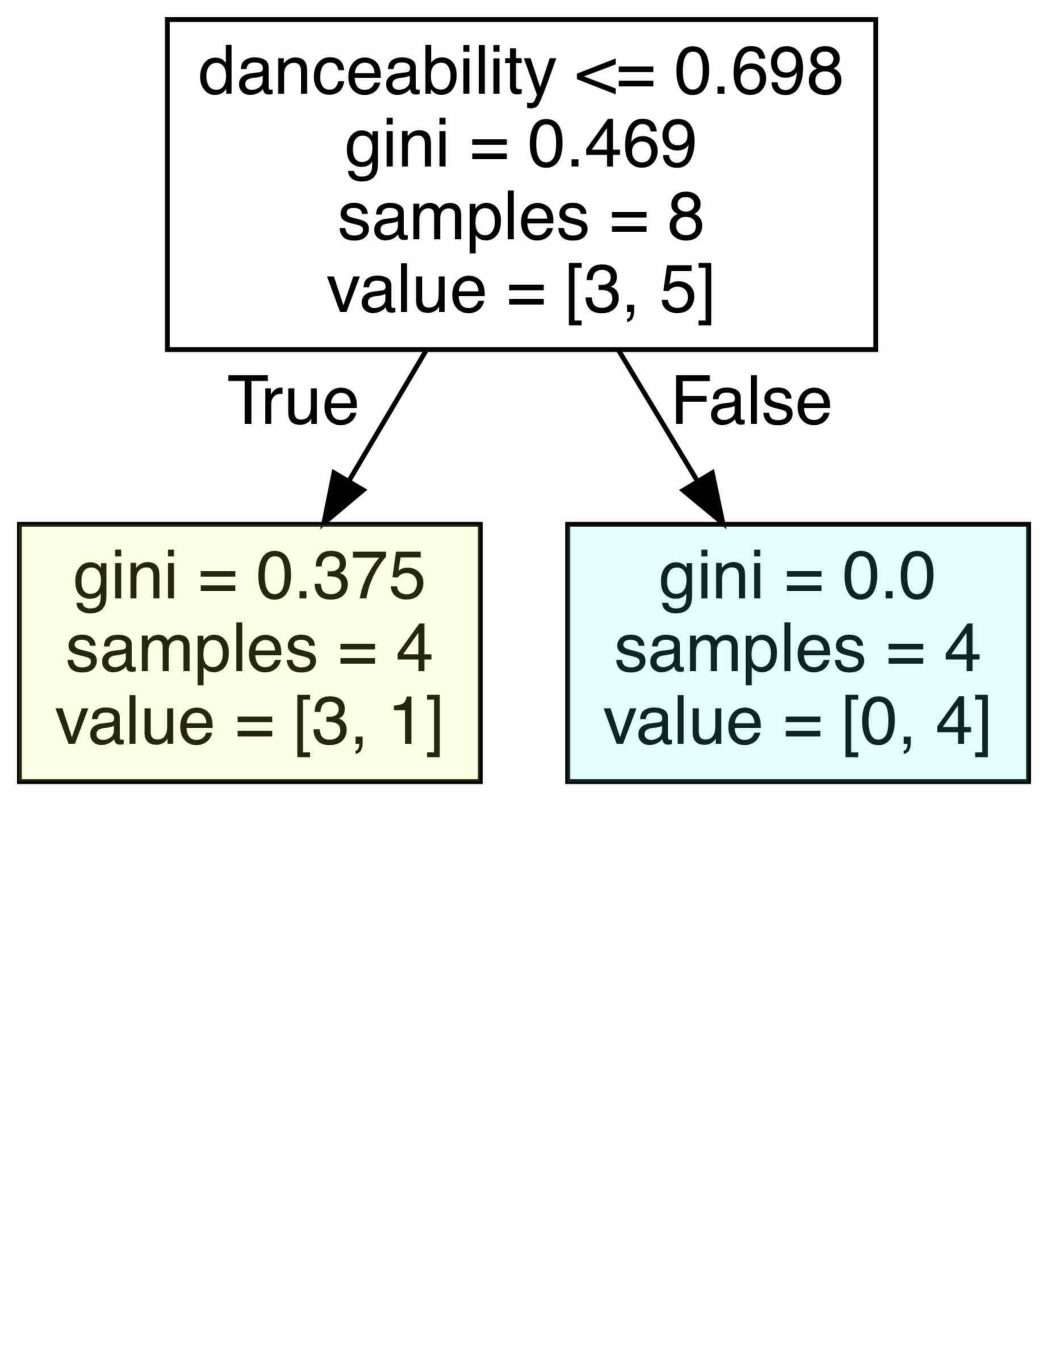
\includegraphics[width=6cm]{dt_first_split.svg.pdf} }}%
    \qquad
    \subfloat[\centering Classification Tree]{{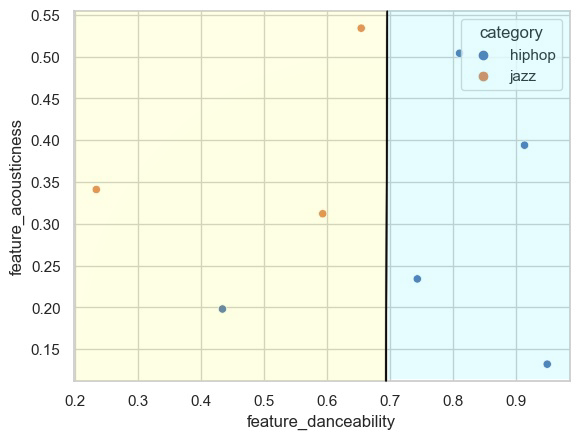
\includegraphics[width=6cm]{coordinate_system_id_first_split.png} }}%
    \caption{Theory: Decision Tree first Split}%
    \label{fig:theory_first_split}%
\end{figure}

\textbf{Stop Criteria:}

The natural stop criterion is a completely homogeneous data-gorup for a node. If a node only contains one single 
class of samples, no further splitting is possible. This is the case for the right node of the example marked in blue. The samples are completely
homogeneous and only consist out of the category \emph{hiphop}. The node therefore automatically becomes a leaf and represents the 
category of samples. Other stop criteria can be predefined depending on own preference. The most relevant criterion is the 
definition of a maximum depth of the decision tree. A maximum depth describes a maximum amount of recurrent iterations before 
the algorithm automatically stops and threats the last nodes as leaves \cite[p.7]{lewis2000introduction}. Maximum depth belongs to a set of hyperparameters that
will be discussed in X and the implementation in more detail chapter. 

\textbf{Completion of the example:}

The second iteration has both nodes created by the first iteration as its input but only the yellow node requires further splitting as 
the blue node is already fully classified. For the second iteration only the feature \emph{acousticness} is relevant as \emph{danceability} cannot 
split this subgroup of the dataset further. The input data for the second split looks like the following (table 2) and the same calculation 
takes place again. 

\begin{table}[H]
    \centering
    \begin{tabular}{llrrr}
        \toprule
        category & track &  feature\_danceability &  feature\_acousticness &  label \\
        \midrule
          hiphop &    h5 &                 0.434 &                 0.198 &      1 \\
            jazz &    j1 &                 0.654 &                 0.534 &      0 \\
            jazz &    j2 &                 0.593 &                 0.312 &      0 \\
            jazz &    j3 &                 0.234 &                 0.341 &      0 \\
        \bottomrule
        \end{tabular}       
    \caption{Theory: Input Data of second Split}%
    \label{tbl:theory_input_data}%
  \end{table} 

  Acousticness: 
  \begin{equation*}
    \begin{aligned}
        Gini^{left} &= 1 - ((\frac{0}{1})^2 + (\frac{1}{1})^2) = 0
        \\
        Gini^{right}  &= 1 - ((\frac{3}{3})^2 + (\frac{0}{3})^2) = 0
        \\
        G(Q_{1},\theta) &= \frac{1}{4} * 0 + \frac{3}{4} * 0 = 0
\end{aligned}
\end{equation*}

This time \emph{acousticness} leads to two fully homogeneous subgroups and thus marks the end of the classification tree as all samples are 
classified correctly. The second split looks like the following with the total classification tree displayed in figure 4.

\begin{figure}[H]
    \centering
    \subfloat[\centering Decision Tree]{{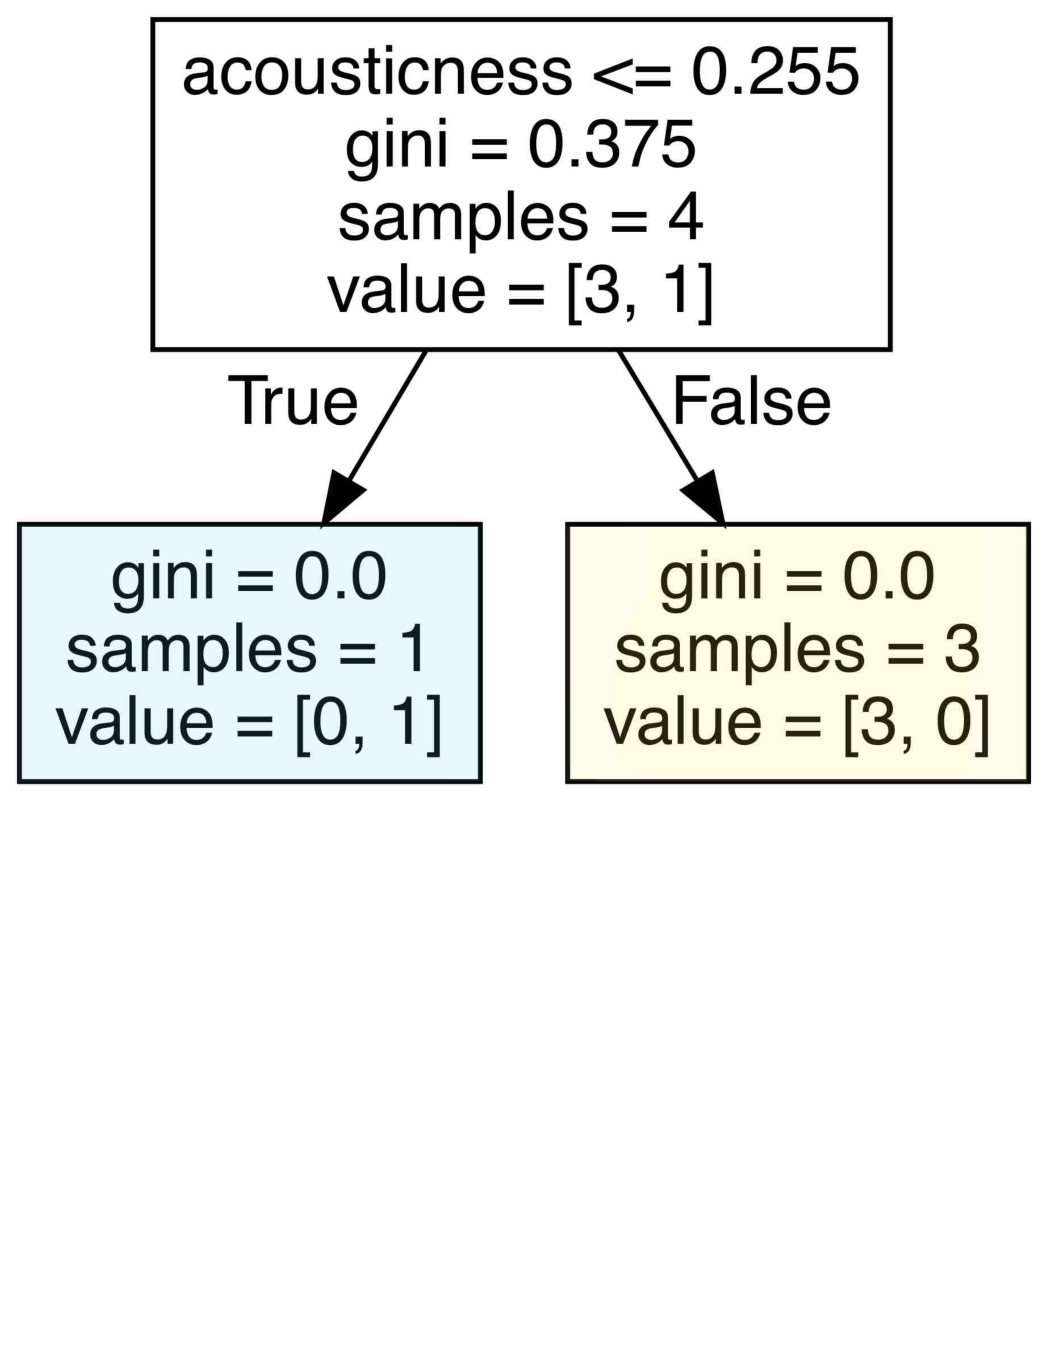
\includegraphics[width=6cm]{dt_second_split copy 2.svg.pdf} }}%
    \qquad
    \subfloat[\centering Classification Tree]{{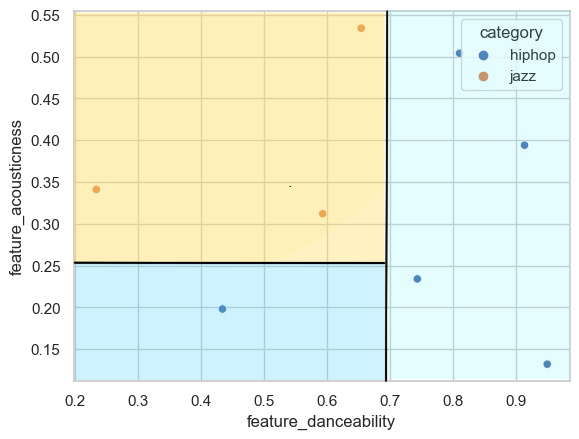
\includegraphics[width=6cm]{coordinate_system_id_second_split.png} }}%
    \caption{Theory: Decision Tree second Split}%
    \label{fig:theory_first_split}%
\end{figure}


\begin{figure}[H]
    \centering
    \caption[]{Theory: Final Classification Tree}
	\label{fig:dt_final_decision_tree}
    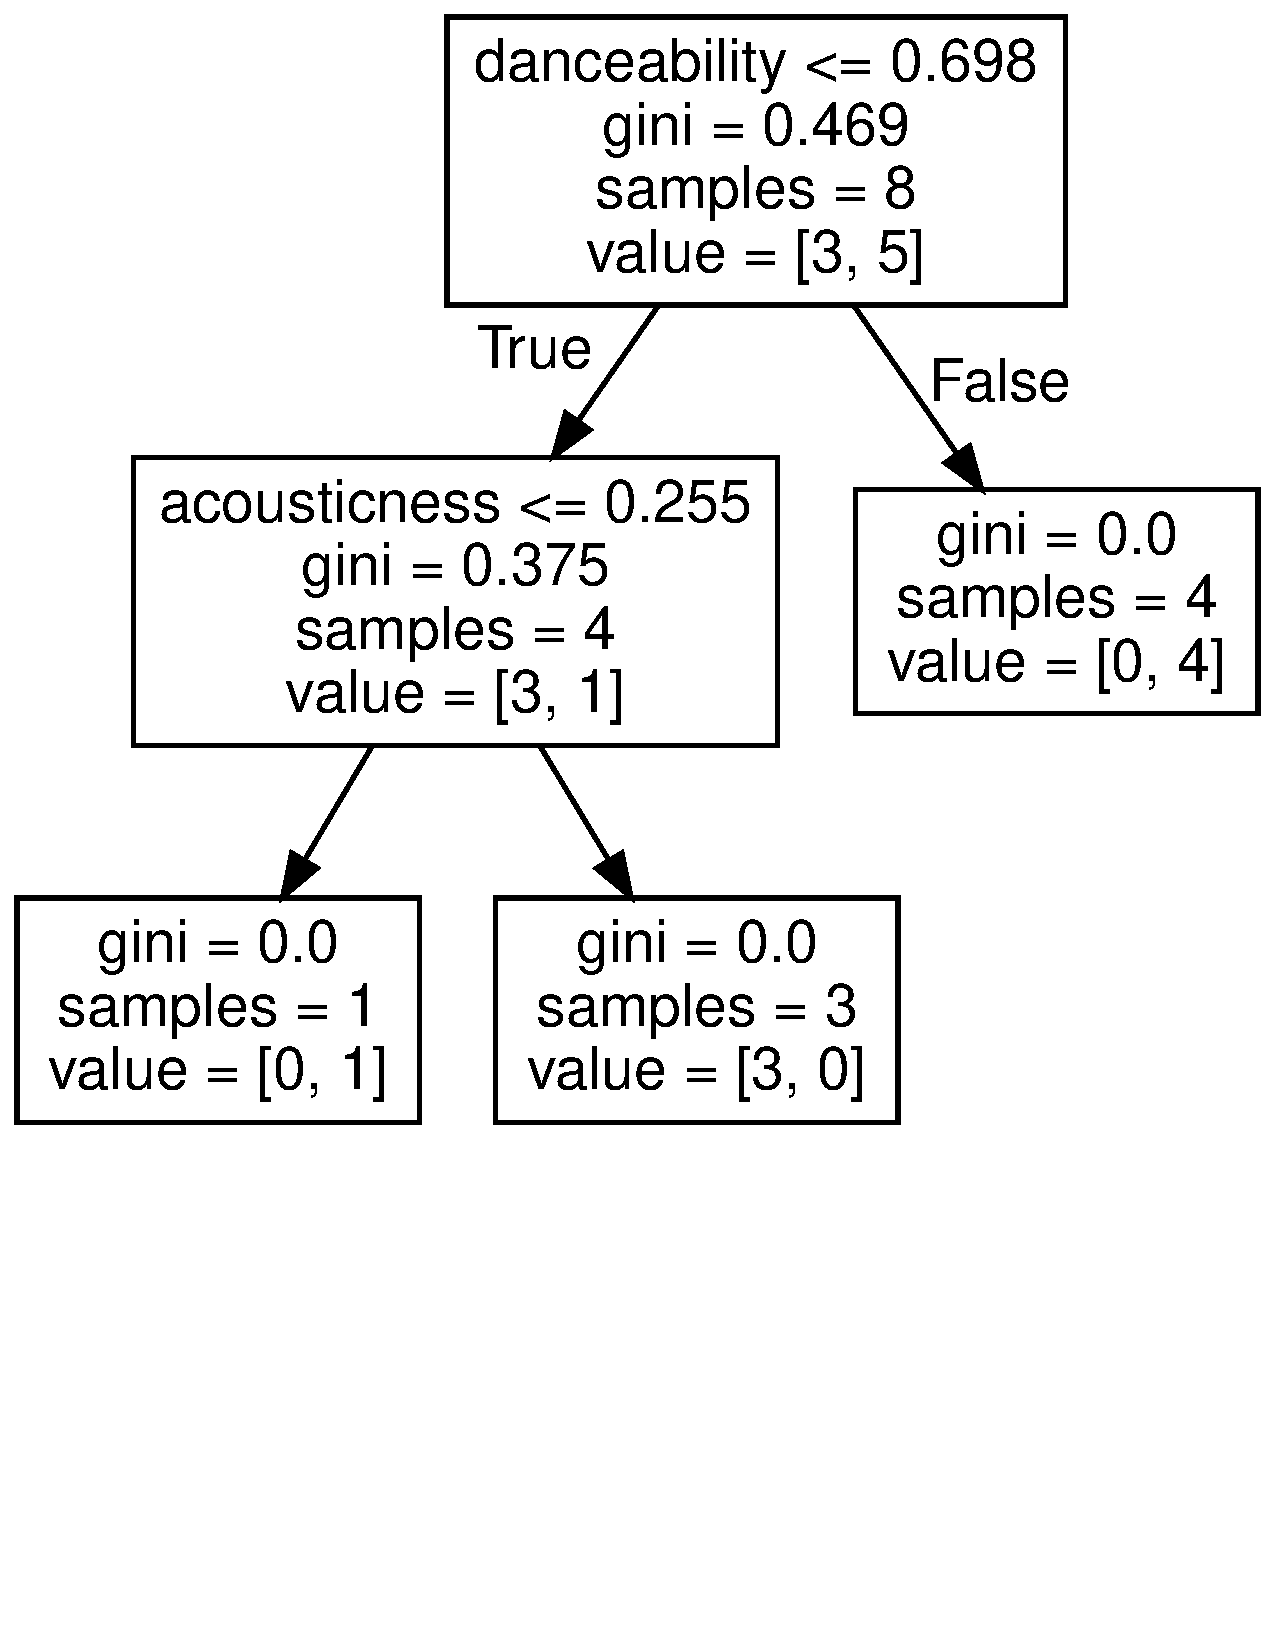
\includegraphics[width=0.58\textwidth]{dt_final_decision_tree.svg.pdf}
\end{figure}

%\textbf{Tree optimization:}
%
%Tree optimization plays a very relevant role because Trees often overclassify training data 
%without countermeasures \cite[p.7]{lewis2000introduction}. Although the training data is well classified, overfitted Decision 
%Trees often produce very poor results for test data. Too accurate classification of training 
%data can negatively affect Decision Trees, as they are less able to generalize the learned 
%knowledge. Pruning is a technique used to overcome overfitting problems by reducing the size of 
%Decision Trees \cite[p.331]{James2021}. Sections that provide little to no classification benefit are removed or not 
%constructed during the recursive splitting process. In essence, worse results for training data 
%are traded for better results for unknown data.

\subsubsection{Evaluation of Decision Trees}

In conclusion, decision trees can be assessed as follows. Starting with the advantages,
the main benefit is the overall simplicity of decision trees, both from a technical and 
business point of view. For researchers and developers, trees are easy to construct, require little
to no data preparation, are almost univerally applicable with a possibility of validation. 
However, the simplicity for business should not be underestimated either. When comparing machine
learning algorithms, the main comparison is often the accuracy of a model. The areas in which 
decision trees stand out include visualization and comprehensibility. The decision tree algorithm 
is a white box model that allows complete transparency and explainability \cite[p.339]{James2021} \cite[10.10.]{sklearn Decision Trees}. 

The disadvantages of decision trees are again closely related to its simplicity. Overfitting and 
the relative instability of decision trees are the main drawbacks and result in good momorization 
but a comparatively weak generalization ability \cite[p.339]{James2021} \cite[10.10.]{sklearn Decision Trees}.

\subsection{Gradient Boosting}

The gradient boosting algorithm is derived from \ac{GBM}, which are a family of 
powerful machine learning algorithms with a certain procedure pattern for the creation of models. 
In general, \ac{GBM}s are very flexible in their characteristics with the possibility of utilizing 
multiple different machine learning algorithms as their foundation.

Boosting differs from classical approaches as it does not consist out of a single predictive 
model but an ensemble approach. Ensemble algorithms contain multiple weak learners that form a 
committee to create a strong prediction. Weak learners are often very simple forms of traditional 
algorithms, like decision trees, and must just be able to predict parts of the dataset correctly. 
Only the combination of many weak learners allows the model to perform overall accurate 
predictions. The most common form of ensemble algorithms are bagging algorithms with random 
forests as an example. Bagging, in essence, is the combination of multiple unique models. The 
prediction is formed by aggregating the outputs from all models into a single representative 
value. Typically, all models are derived from a single algorithm, like decision trees for random 
forests, but technically there is no limitation to aggregate outputs from different algorithms. 
Which is also true for other ensemble algorithms. 

Boosting, on the other hand, follows a different principle and does not rely on independent 
models with an aggregation function. Boosting fits new models sequentially and can thereby use 
earlier acquired knowledge for further iterations. This allows GBMs to train specific areas of 
the dataset where it has previously performed poorly \cite[p.345f]{James2021}.  

\subsubsection{Gradient Boosting Algorithm}
\label{sec:Gradient Boosting Algorithm}

The generic gradient boosting algorithm follows a sequence of three steps beginning with the initalization of
of the dataset, over the sequential training and ending with a final output. At the beginning, an 
additional initiation of the dataset and a loss function is necessary. The mathematical 
representation of the dataset is like the one used for decision tees. A summary: \(x_{i}\) present the 
explanatory features while \(y_{i}\) represents the corresponding label for one data point of the input 
dataset \(N\) with a total number of \(n\) samples. 

The mathematical goal of the algorithm is to reconstruct the unknown functional dependance \(f\) 
between \(x_{i}\) and \(y_{i}\) with an estimate \(F^{*}\) for every data point, such that the specific Loss 
Function \(L(y, \gamma)\) is minimized (5) \cite[p.1189]{Friedman_2001} \cite[2.1]{Natekin2013}. 

\begin{equation}
F^{*} = \arg \min_{\gamma} L(y,\gamma)
\end{equation}

\textbf{Loss Function and Weak Learners:}

The loss function is an indicator for the quality of the model. A small loss for a data point 
means that the prediction is close or identical to the observed label and the model therefore 
categorizes the sample correctly whereas a high loss implies that the model could not predict 
the sample well. Given a particular learning task and dataset, different loss functions must 
be considered as loss functions are only suitable for specific data and task constellations. The most common 
loss function for binary classification is the so-called bernoulli loss (6). The bernoulli loss 
can be transformed into a \(log(odds)\)-prediction (7) as it is better suited for further calculations. 
Variations of (7) will be used in the following section to demonstrate the gradient boosting 
procedure \cite[3.1]{Natekin2013}. 

\begin{equation}
L(y_{m}, \gamma) = - log(likelihood)
\end{equation} 

\begin{equation}
L(y_{m}, \gamma) = - y_{i} * log(odds) - log(1-p)
\end{equation}

Additionally, a machine learning algorithm must be defined as a weak learner. For \ac{GBM}s there 
are multiple leaners to choose from, again the choice is mostly depending on the prediction 
task and available data \cite[3.2]{Natekin2013}. A classical approach is the use of decision trees, which was also 
chosen as the weak learner for this project. Decision trees used for gradient boosting are 
always regression trees, regardless of whether they are used for regression or classification 
problems. The optimization parameters are almost identical as for standalone decision trees, 
but the trees often look very different because they are specifically created as weak learners. 
As a result, the decision trees often only consist out of very few layers with only 8-32 leaves.
(QUELLE)

\textbf{1. Initialization:}

To showcase the gradient boosting algorithm the same sample dataset is used as for decision trees. 
It again consists out of eight samples with two features and two categories as target Labels. 

\begin{table}[H]
    \centering
    \begin{tabular}{llrrr}
        \toprule
        category & track &  feature\_danceability &  feature\_acousticness &  label \\
        \midrule
          hiphop &    h1 &                 0.949 &                 0.132 &      1 \\
          hiphop &    h2 &                 0.743 &                 0.234 &      1 \\
          hiphop &    h3 &                 0.913 &                 0.394 &      1 \\
          hiphop &    h4 &                 0.810 &                 0.504 &      1 \\
          hiphop &    h5 &                 0.434 &                 0.198 &      1 \\
            jazz &    j1 &                 0.654 &                 0.534 &      0 \\
            jazz &    j2 &                 0.593 &                 0.312 &      0 \\
            jazz &    j3 &                 0.234 &                 0.341 &      0 \\
        \bottomrule
        \end{tabular}        
    \caption{Theory: Input Data}%
    \label{tbl:theory_input_data}%
  \end{table} 

The first step is to set an initial prediction for all samples of the dataset. The initial 
prediction is not unique for individual samples but a uniform value. The optimal initial 
prediction can be calculated using the following equation (8). For \(F_{0}(x)\), representing the 
initial prediction, a minimum of \(\gamma \) is searched for. The right-hand side of the equation 
only consists out of a sum for each sample \(i\) (of the total dataset \(N\)) of the known loss function 
with the respective label \(y_{i}\) and \(\gamma \) as its input. To find the low point of the equation, 
the derivate of the loss function is required. The final calculation of the overall \(log (odds)\) 
that a song is classified as \emph{hiphop} is the \(\log_{e}\) of the sum of songs of the category \emph{hiphop}
divided by the sum of the songs of the category \emph{jazz}. The result can be checked graphically 
as is equal to the \(x1\)-coordinate value of the low point of the \(log(odds)\)-prediction (figure 5). 

\begin{equation}
    F_{0}(x) = \arg \min_{\gamma } \sum_{i= 1}^{n} L(y_{i}, \gamma)
\end{equation}

\begin{equation*}
    F_{0}(x) = \log_{e}(\frac{5}{3}) = 0.51
\end{equation*}

\begin{figure}[H]
    \centering
    \caption[]{Theory: Gradient Boosting Minimum for first Prediction}
	\label{TurningPoint-LossFunctio}
    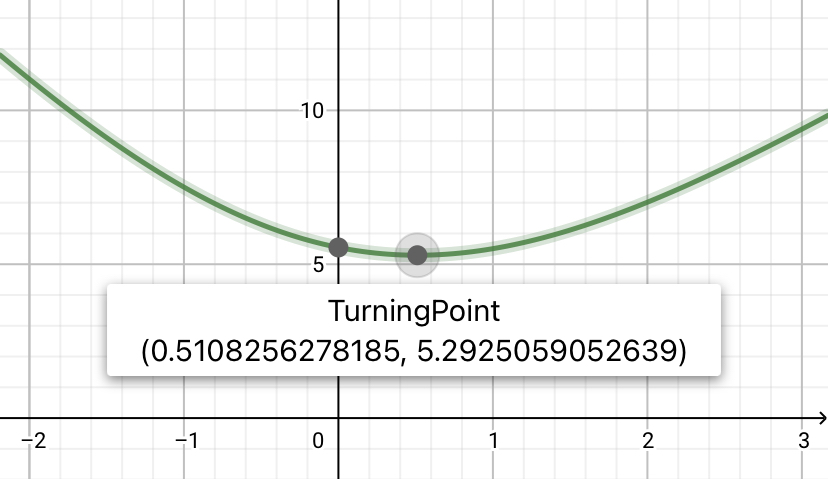
\includegraphics[width=0.5\textwidth]{TurningPoint-LossFunction.jpeg}
\end{figure}

\textbf{2. Sequential Processing:}

With the completion of the initialization of the dataset the modelling can begin. The training is a sequential 
process of constructing the regression trees with a total of \(M\) iterations. The first iteration 
starts with \(m = 1\). The modelling consists out of four sub-steps which are numbered consecutively.

First, the \(log(odds)\)-prediction must be converted back into a probability \(p\) with the help of a 
logistic function as probability is easier to use for classification (9). The result is 
that all songs have the probability of \(0,63\) to belong to the category \emph{hiphop}.

\begin{equation}
p = \frac{e^{\log_{e}(odds)}}{1 + e^{\log_{e}(odds)}} 
\end{equation}

\begin{equation*}
p = \frac{e^{\log_{e}(\frac{5}{3})}}{1 + e^{\log_{e}(\frac{5}{3})}} = 0,63
\end{equation*}

In the \textbf{first step} the \ac{PR}s \(r_{im}\) for each sample \(i\) of the dataset are created. The equation (10) 
for calculating the \ac{PR} consists out of known fragments. For every sample \(i\) a PR \(r_{im}\) 
is calculated using the derivative of the \(log(odds)\)-prediction with the label \(y_{i}\) and the 
prediction of the last iteration \(F = F_{m - 1}\) as its input. Again, the equation can be 
transformed into a very simple equation. For each sample the \ac{PR} can be calculated by only 
subtracting the previously calculated probability \(p\) from the observed label \(y\). Ideally, an additional 
column is created in which the PRs are temporarily stored (table 4). 

\begin{equation}
    \begin{aligned}
        r_{im} &= - (\frac{\partial L(y_{i}, F(x_{i}))}{\partial F(x_{i})})_{F = F_{m - 1}}
        \\
        r_{im} &= (y_{i} - p_{i})
    \end{aligned}
\end{equation}

This and every following calculation is explained for the track \emph{h1} of the dataset while the result for 
every other sample will be shown in form of a table. 

\begin{equation*}
r_{1,1} = 1 - 0.625 = 0.375
\end{equation*}

\begin{table}[H]
    \centering
    \begin{tabular}{llrrrr}
        \toprule
        category & track &  label & \(F_{0}(x)\) &  probability \(F_{0}(x)\) &  pseudo residuals \\
        \midrule
          hiphop &    h1 &      1 & 0.510826 &         0.624988 &            0.375012 \\
          hiphop &    h2 &      1 & 0.510826 &         0.624988 &            0.375012 \\
          hiphop &    h3 &      1 & 0.510826 &         0.624988 &            0.375012 \\
          hiphop &    h4 &      1 & 0.510826 &         0.624988 &            0.375012 \\
          hiphop &    h5 &      1 & 0.510826 &         0.624988 &            0.375012 \\
            jazz &    j1 &      0 & 0.510826 &         0.624988 &           -0.624988 \\
            jazz &    j2 &      0 & 0.510826 &         0.624988 &           -0.624988 \\
            jazz &    j3 &      0 & 0.510826 &         0.624988 &           -0.624988 \\
        \bottomrule
        \end{tabular} 
    \caption{Theory: Pseudo Residuals for first Iteration}%
    \label{tbl:theory_pseudo_residuals_1_iteration}%
  \end{table} 

The \textbf{second step} constructs the regression trees out of the features of the samples with the corresponding 
PR as the label. For this example, only tree stumps are created to simplify the implementation. 
The regression tree for the first iteration is shown in figure 6. After the completion of the 
tree, terminal regions \(R_{jm}\) must be defined for every leaf. \(j\) starts with \(1\) and is increased for 
every leaf \cite[p.1195]{Friedman_2001}. 

\begin{figure}[H]
    \centering
    \caption[]{Theory: Regression Tree for first Iteration}
	\label{gb_1_regression_tree}
    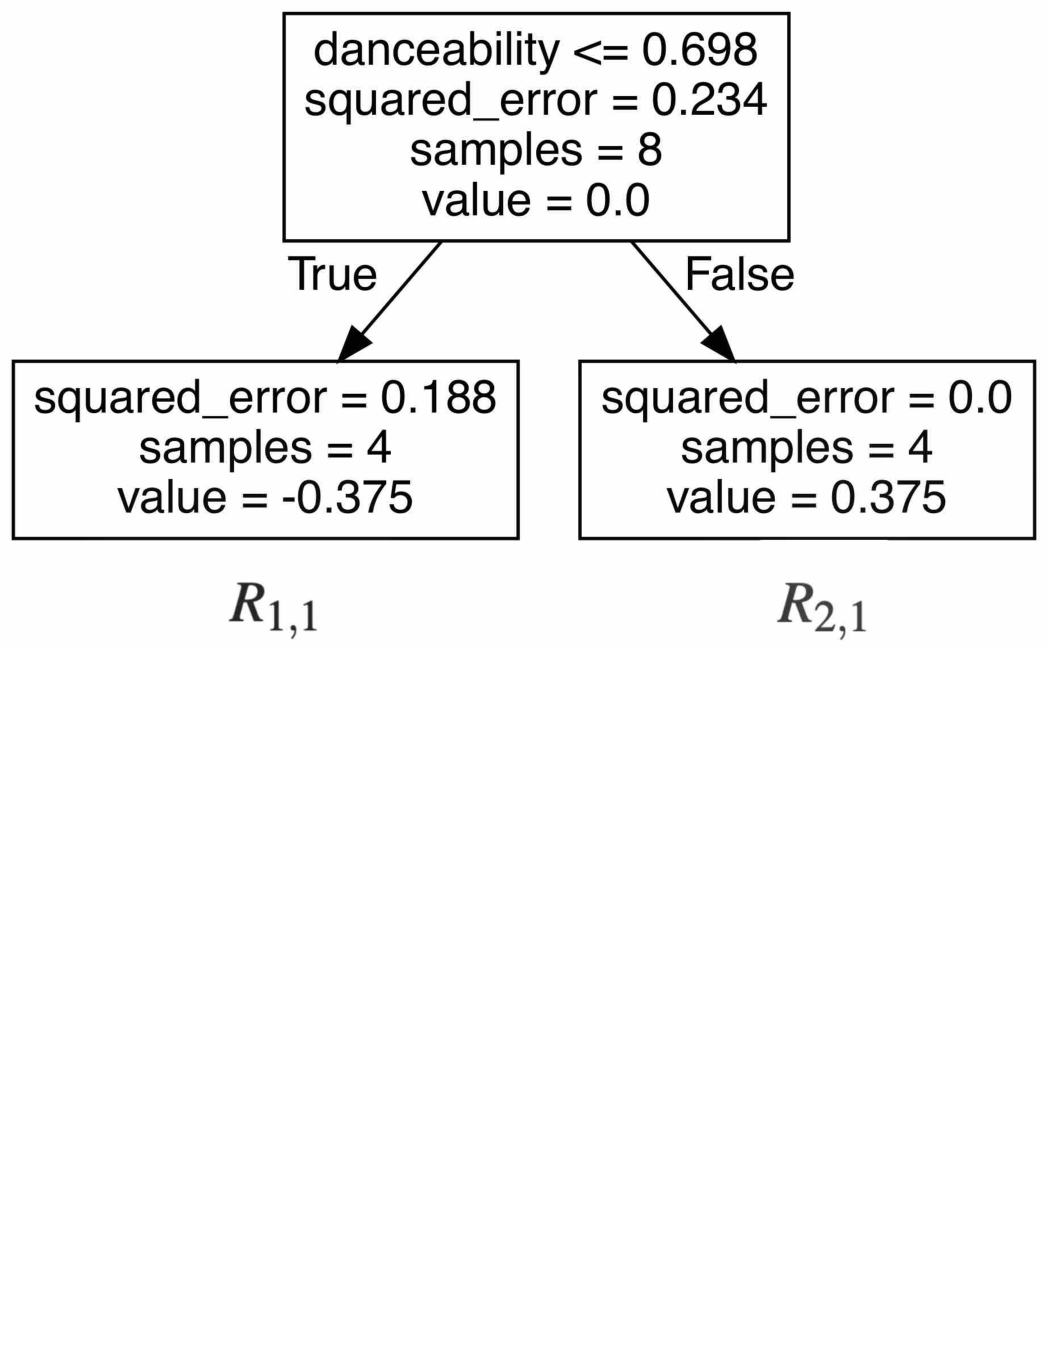
\includegraphics[width=0.5\textwidth]{gb_1_regression_tree.svg.pdf}
\end{figure}

In \textbf{step three}, following the completion of the regression tree, output values \(\gamma_{j, m}\) are calculated by using 
the equation presented in (10). For each leaf in the tree \(\gamma_{j, m}\) is computed by finding 
\(\gamma_{j, m}\) that minimizes the loss function (11). Like for the initialization step, the derivative has 
to be created and must set equal to \(0\). And again, after a complicated transformation, a very simple 
equation remains (11). The \(\gamma_{j, m}\)  can be calculated using only the \ac{PR} and the most 
recent predicted probabilities \(p\) for all samples in the leaf. 

\begin{equation}
    \begin{aligned}
        \gamma_{jm} &= \arg \min_{\gamma}\sum_{x_{i} in R_{ij}} L(y_{i},F_{m-1}(x_{i} + \gamma))
        \\
        \gamma_{jm} &= \frac{ \sum r_{im}}{\sum p_{i} * (1 - p_{i})}
    \end{aligned}
\end{equation}

For \(R_{2,1}\), which contains track \emph{h1}, the calculation looks like the following. The output values of the complete 
dataset are displayed in table 5. 

\begin{equation*}
\gamma_{\;2,1} = \frac{0.375\;*\;4}{(\:0.625\;*\;(1\;-\;0.625))\;*\;4} = 1.6 
\end{equation*}

\begin{table}[H]
    \centering
    \begin{tabular}{llrrrr}
        \toprule
        category & track &  label &  \(F_{0}(x)\) &  pseudo residuals &  output value \\
        \midrule
          hiphop &    h1 &      1 & 0.510826 &            0.375012 &        1.600032 \\
          hiphop &    h2 &      1 & 0.510826 &            0.375012 &        1.600032 \\
          hiphop &    h3 &      1 & 0.510826 &            0.375012 &        1.600032 \\
          hiphop &    h4 &      1 & 0.510826 &            0.375012 &        1.600032 \\
          hiphop &    h5 &      1 & 0.510826 &            0.375012 &       -1.599926 \\
            jazz &    j1 &      0 & 0.510826 &           -0.624988 &       -1.599926 \\
            jazz &    j2 &      0 & 0.510826 &           -0.624988 &       -1.599926 \\
            jazz &    j3 &      0 & 0.510826 &           -0.624988 &       -1.599926 \\
        \bottomrule
        \end{tabular}
    \caption{Theory: Output Values for first Iteration}%
    \label{tbl:theory_output_values_1_iteration}%
  \end{table} 

\textbf{Step four} marks the end of the first iteration and creates a new prediction \(F_{m}(x)\) for each sample. 
The new \(log(odds)\)-prediction is based on the last \(log(odds)\)-prediction plus the learning rate \(\nu\) multiplied by 
the output values for the sample of the last regression tree (12) \cite[p.1203]{Friedman_2001}. Normally, there is only one 
output value for a sample which makes the summation sign obsolete. The learning rate \(\nu\) is a 
hyperparameter for gradient boosting. For this example, a high \(\nu\) of \(0.6\) is used to better visualize 
the changes. In practice a \(\nu \) in the order of \(0.1\) is common as a small learning rate tends to
give better results but also requires much more iterations \cite[p.1206]{Friedman_2001}. 

\begin{equation}
F_{m}(x) = F_{m}(x- 1) + \nu * \sum_{j = 1}^{J_{m}} \gamma_{jm}I(x in R_{jm})
\end{equation}

The prediction \(F_{1}(x)\) for \emph{h1} looks as follows while the complete dataset is again displayed in table 6 with also 
the probabilites shown. As one can see, the probabilites for most samples got closer to the label. However, for track
\emph{h5} the prediciton got worse. This is why multiple iterations are necessary to form a well-founded prediction. 

\begin{equation*}
F_{1}(x) = 0.51 + 0.6 * 1.6 = 1.47
\end{equation*}


\begin{table}[H]
    \centering
    \begin{tabular}{llrrrrr}
        \toprule
        category & track &  label & \(F_{0}(x)\) &  probability \(F_{0}(x)\) &  \(F_{1}(x)\) &  probability \(F_{1}(x)\) \\
        \midrule
          hiphop &    h1 &      1 & 0.510826 &         0.624988 &  1.470845 &         0.813163 \\
          hiphop &    h2 &      1 & 0.510826 &         0.624988 &  1.470845 &         0.813163 \\
          hiphop &    h3 &      1 & 0.510826 &         0.624988 &  1.470845 &         0.813163 \\
          hiphop &    h4 &      1 & 0.510826 &         0.624988 &  1.470845 &         0.813163 \\
          hiphop &    h5 &      1 & 0.510826 &         0.624988 & -0.449130 &         0.389579 \\
            jazz &    j1 &      0 & 0.510826 &         0.624988 & -0.449130 &         0.389579 \\
            jazz &    j2 &      0 & 0.510826 &         0.624988 & -0.449130 &         0.389579 \\
            jazz &    j3 &      0 & 0.510826 &         0.624988 & -0.449130 &         0.389579 \\
        \bottomrule
        \end{tabular}
    \caption{Theory: Output Values for first Iteration}%
    \label{tbl:theory_output_values_1_iteration}%
  \end{table} 

The second iteration of the modelling phase follows the exact same principles and will again be showcased for track \emph{h1}. 
It marks the end for this example. 

\begin{itemize}

    \item New probability:

    \begin{equation*}
        p = \frac{e^{1.47}}{1 + e^{1.47}} = 0,81
    \end{equation*}

    \item New pseudo residuals: 

    \begin{equation*}
        r_{1, 2} = 1 - 0.81 = 0.19
    \end{equation*}
    
    \item New decision tree with terminal regions:

    \begin{figure}[H]
        \centering
        \caption[]{Gradient Boosting: Second Regression Tree}
        \label{gb_2_regression_tree}
        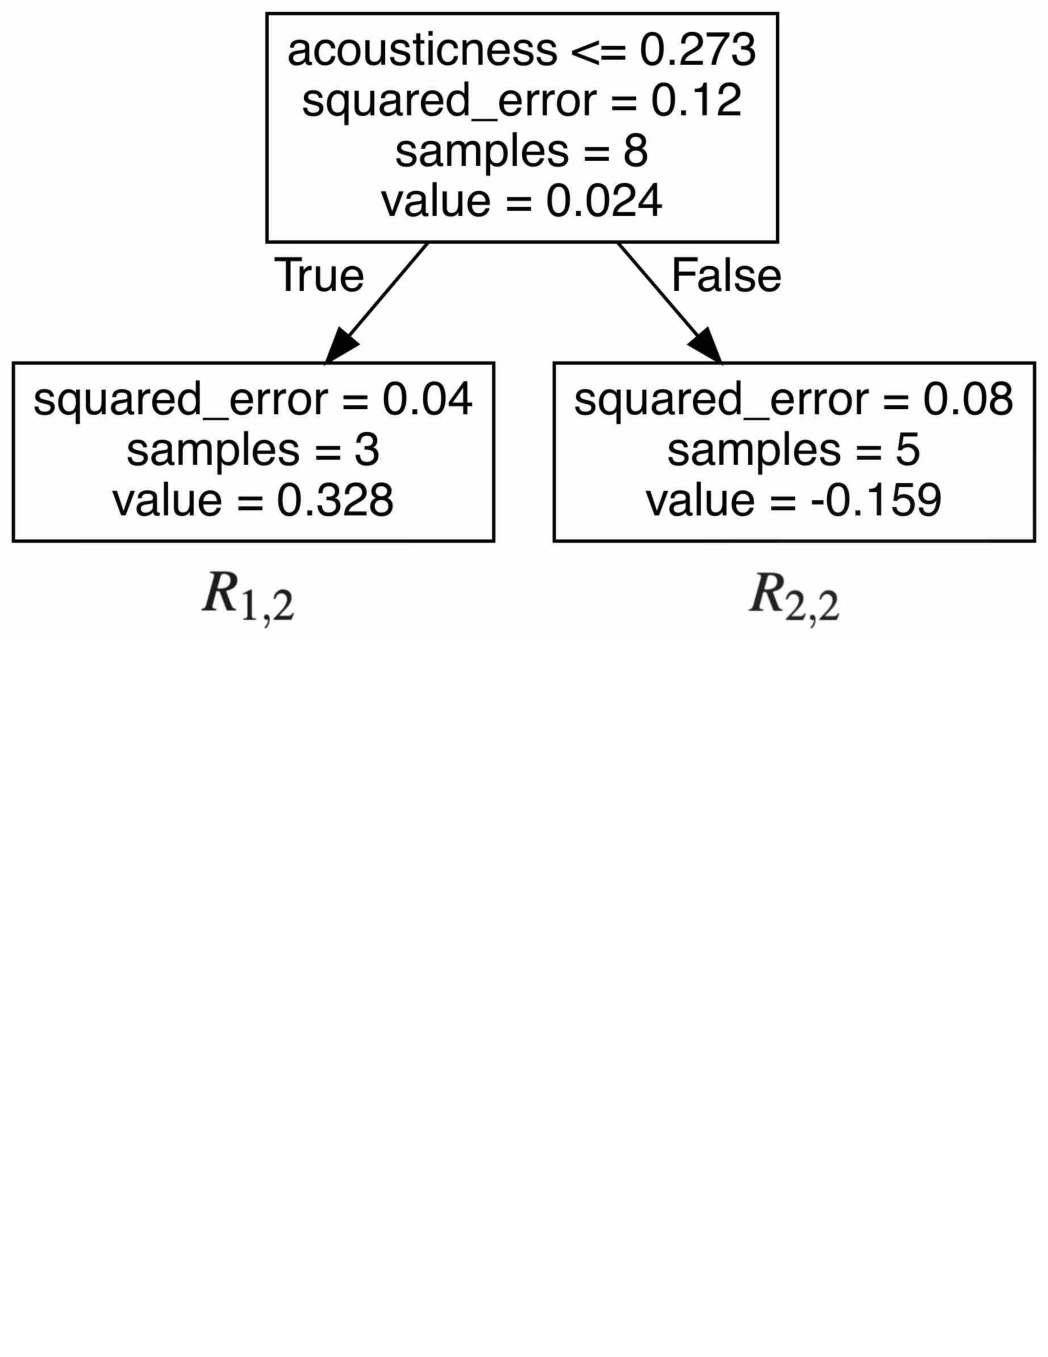
\includegraphics[width=0.5\textwidth]{gb_2_regression_tree.svg.pdf}
    \end{figure}

    \item New output value: 

    \begin{equation*}
        \gamma_{\;2,2} = \frac{0.98}{0.54} = 1.81 
    \end{equation*}

    \item New prediction:

    \begin{equation*}
        F_{2}(x) = 1.47 + 0.6 * 1.81 = 2.56
    \end{equation*}

    \item New probability:

    \begin{equation*}
        p = \frac{e^{2.56}}{1 + e^{2.56}} = 0.93 
    \end{equation*}

\end{itemize}

The iterative modelling is repeated until \(M\) is reached. \(M\) marks the completion of the training of the gradient 
boosting model. The \(F_{M}(x)\) is the final prediction for every sample. Lastly, the predicitions
must again be transformed to probabilites like for the calculation of the \ac{PR}. For the final probabilities 
thresholds are used to compute the category to which the samples belong \cite[p.1204]{Friedman_2001}. A typical threshold 
for binary classification is \(0.5\) as it splits \(F_{M}(x)\) into two equal classes.

\textbf{3. Output:}

Sample \emph{h1} has a final probability of \(0.93\) of belonging to the category \emph{hiphop}. \(0.93\) is by far greater than the 
predefined threshold of \(0.5\) and thus \emph{h1} is classified as a track that belongs to the category \emph{hiphop}. Table 7 shows
that all samples are classified correctly but some less clear than others. A real-world implementation would consist 
out of more iterative models with different regression trees and a different learning rate to enhance the 
classification potential. Also the dataset would be very different with more samples that consist out of more features. 

\begin{table}[H]
    \centering
    \begin{tabular}{llrrrrr}
        \toprule
        category & track &  prob. \(F_{0}(x)\) &    \(F_{1}(x)\) &  prob. \(F_{1}(x)\) &       \(F_{2}(x)\) &  Output Probability \\
        \midrule
          hiphop &    h1 &         0.624988 &  1.470845 &         0.813163 &  2.560923 &                          0.928286 \\
          hiphop &    h2 &         0.624988 &  1.470845 &         0.813163 &  2.560923 &                          0.928286 \\
          hiphop &    h3 &         0.624988 &  1.470845 &         0.813163 &  1.001911 &                          0.731414 \\
          hiphop &    h4 &         0.624988 &  1.470845 &         0.813163 &  1.001911 &                          0.731414 \\
          hiphop &    h5 &         0.624988 & -0.449130 &         0.389579 &  0.640948 &                          0.654953 \\
            jazz &    j1 &         0.624988 & -0.449130 &         0.389579 & -0.918064 &                          0.285372 \\
            jazz &    j2 &         0.624988 & -0.449130 &         0.389579 & -0.918064 &                          0.285372 \\
            jazz &    j3 &         0.624988 & -0.449130 &         0.389579 & -0.918064 &                          0.285372 \\
        \bottomrule
        \end{tabular}           
    \caption{Theory: Gradient Boosting final Output}%
    \label{tbl:theory_gb_final_output}%
  \end{table} 

An unknown sample gets initialized by \(F_{0}(x)\) and is sequentially routed through every model. For each iteration the 
Prediction is updated using the output value of the regression tree. Finally, the last probability is used to classify 
the sample using the predefined threshold. 

\subsubsection{Evaluation of Gradient Boosting}

Gradient boosting is a very powerful method as it can effectively capure complex dependencies for various machine 
learning problems. \ac{GBM}s improve many existing algorithms, such as decision trees, because many problems associated 
with single large models are (partially) solved by the iterative ensemble approach. 

The main benefit over Decision Trees is the stability of gradient boosting. While large trees always have to make tradeoffs 
between detail and overcategorization, gradient boosting can gradually get to a deeper and deeper level of detail thanks to 
small trees with overall better generalization. Furthermore the flexbility of gradient boosting and boosting in general is massive 
as it only represents the framework with many parameters to adapt the algorithm very specifically to the usecase.  

The drawbacks of gradient boosting often arise in practice. Gradient boosting has a significantly higher memory consumption and 
build time as the model must be constructed sequentially. Also the evalutation is more time consuming as the sample must be processed 
by each model. From a business perspective gradient boosting also has its disadvantages. While the prediciton is better, it is much 
more complex to evaluate the model and explain the results \cite[7.2]{Natekin2013}. 